\documentclass[11pt]{article}
\usepackage[italian]{babel}
\usepackage[utf8]{inputenc}
\usepackage{graphicx}
\usepackage{float}
\usepackage{amsmath}
\usepackage{amsfonts}
\usepackage{hyperref}
\usepackage{fontspec}
\usepackage{glossaries}
\makeglossaries
\newglossaryentry{magic}{
    name={magic number},
    description={quel numero che metti in una variabile quando è nulla ma non hai il null. Tipo -1}
}
\newglossaryentry{agnostic}{
    name={platform agnostic},
    description={intendiamo software che può essere eseguito allo stesso modo su diverse piattaforme}
}
\newglossaryentry{lifo}{
    name={LIFO},
    description={con logica Last In, First Out}
}
\newglossaryentry{fifo}{
    name={FIFO},
    description={con logica First In, First Out}
}
\newglossaryentry{constraint}{
    name={constraint},
    description={un constraint è un limite che viene posto; restriction, limitation.}
}
\newglossaryentry{statement}{
    name={statement},
    description={istruzioni del codice e.g. una riga di codice}
}
\newglossaryentry{mock}{
    name={mock},
    description={da Wikipedia: \textit{"Nella programmazione orientata agli oggetti, i mock object (simulati o mock object) sono degli oggetti simulati che riproducono il comportamento degli oggetti reali in modo controllato. Un programmatore crea un oggetto mock per testare il comportamento di altri oggetti, reali, ma legati ad un oggetto inaccessibile o non implementato. Allora quest'ultimo verrà sostituito da un mock."}}
}
\usepackage[normalem]{ulem}
\setmainfont{[SansForgetica-Regular.otf]}
\newcommand{\code}[1]{\texttt{#1}}
\newcommand{\numpy}{{\tt numpy}}    % tt font for numpy
\topmargin -.5in
\textheight 9in
\oddsidemargin -.25in
\evensidemargin -.25in
\textwidth 7in
\begin{document}

% ========== Edit your name here
\author{Simone Montali\\monta.li}
\title{Riassunti di Ingegneria del Software}

\maketitle

\medskip
\section*{Prefazione}
Questo progetto nasce dalla necessità di trovare un metodo di studio per questa materia che, ai più sembra banale. Il problema di fondo è proprio in questa apparente banalità: si finisce per studiarla di fretta pensando di conoscerla, e ci si rende conto troppo tardi di non essere pronti. Mi scuso, anzitutto, per il vocabolario misto italiano-inglese che utilizzerò in queste pagine. Tanti di voi sanno quanto sia complicato esprimere certi concetti in italiano. Ho inserito un piccolo glossario a fine documento. Questo documento ha lo scopo di essere il giusto mezzo tra completezza e sinteticità. Mi scuso, in secundis, per i toni a volte scurrili. Un vero informatico è arrabbiato \textit{/per il codice che non compila/\LaTeX  che fa ciò che vuole/il computer che si impalla/quel piccolo bugfix di Linux che diventa un bagno di sangue/}, e non c'è modo migliore di sfogare le incazzature informatiche che imprecare in riassunti che leggeranno le generazioni a venire. 
Non so come tu ti sia procurato questo documento, ma se hai 5 minuti da buttare, dai una letta alle cose che ho scritto \href{https://monta.li/appunti}{qui.} Ci troverai anche un'altra valangata di appunti. Buona studiata ed in bocca al lupo per tutto.
\section{J1 - Java Overview}
Java è un linguaggio object-oriented, derivato da C/C++, nato per applicazioni web. È semplice, multi-threaded, dinamico. Ha ereditato da C++ la sintassi. Vi sono però alcune differenze: mancanza di puntatori, garbage collection, mancanza di header files e preprocessori. Rispetto a C++, si avvia più velocemente, richiede meno codice, è indipendente dalla piattaforma e più facile da distribuire. Esistono 3 versioni:
\begin{itemize}
    \item Java Standard Edition (J2SE): applicazioni stand-alone client-side
    \item Java Enterprise Edition (J2EE): applicazioni server-side
    \item Java Micro Edition (J2ME): utilizzato per dispositivi piccoli, come i cellulari
\end{itemize}
Il software viene eseguito sulla \textbf{Java Virtual Machine}, che permette di essere indipendente dalla piattaforma. I file .java contengono i sorgenti, i file .class il codice compilato (\textit{bytecode}). Un file jar contiene il bytecode e i file multimediali, e viene utilizzato per distribuire l'applicazione. 
\subsection{Serializzazione e riflessione}
La serializzazione è il meccanismo che converte oggetti in \textbf{byte streams}. La deserializzazione è il processo inverso. Questo meccanismo è utilizzato per trasferire e salvare oggetti. La \textbf{riflessione} permette a un programma di analizzarsi e manipolare le sue proprietà interne.
\subsection{JRE e JDK}
Il \textbf{Java Runtime Environment} è un pacchetto software contenente la JVM, alcuni librerie (.jar) e altri componenti. Il suo scopo è eseguire applicazioni scritte in Java. Il \textbf{Java Development Kit} è un superset, contenente gli strumenti atti a sviluppare, debuggare e monitorare le applicazioni. 
\subsection{Platform Module System}
Introdotto da Java9, aggiunge un livello di aggregazione oltre ai pacchetti: i \textbf{moduli}. Un modulo definisce un gruppo riutilizzabile di pacchetti e risorse (immagini/XML/...). Un modulo ha bisogno di \textit{Java Module Descriptor}, module-info.java, contenuto nella root del modulo. Può anche dipendere da altri moduli, ma aciclicamente.
Le sue caratteristiche principali sono:
\begin{itemize}
    \item Configurazione affidabile: la modularità permette di dichiarare con chiarezza le dipendenze
    \item Forte incapsulamento: i pacchetti in un modulo sono accessibili solo se esportati
    \item Piattaforma Java scalabile: la piattaforma java include tanti moduli, ma si può creare dei custom runtime per caricare solo i moduli necessari
\end{itemize} 
Il \textbf{module descriptor} include nome, dipendenze, pacchetti esportati, servizi forniti, servizi utilizzati, e una lista dei moduli che sfruttano la reflection.
\subsection{Garbage collector}
Il \textbf{garbage collector} controlla la memoria e trova quali oggetti non sono più "referenziati" da variabili, per eliminarli. Inoltre, compatta gli oggetti rimanenti. Il GC non può essere invocato esplicitamente, ma si può suggerire alla JVM di farlo girare.
\section{J2 - Development tools}
\begin{itemize}
    \item \textbf{Eclipse} è l'IDE che va per la maggiore su Java. È una piattaforma aperta, espandibile con plugin, che fornisce tool per programmare, compilare, debuggare. 
    \item \textbf{Papyrus} è un editor UML basato su Eclipse, fortemente incentrato sulla customizability. Supporta anche i constraint OCL (vedi T12).
\end{itemize}
\subsection{Build tools}
I \textbf{build tools} vengono utilizzati per compilare e costruire immagini software dal source code. Richiedono due componenti: un build script che definisce le task da eseguire, ed un eseguibile che lo processa. Gli script dovrebbero essere \gls{agnostic}.
\subsubsection{Maven}
\textbf{Maven} è un tool di software project management che fornisce un setup di progetto semplice, con dipendenze e management di release e distribuzione. Incoraggia l'uso di una repository centrale di JAR e dipendenze. Permette la scrittura di plugin. I build files sono scritti in XML utilizzando il formato \textit{Project Object Model} (POM), i pom.xml.
\subsection{Static Analysis Tools}
Questi tool possono trovare bug ispezionando il codice senza eseguirlo. Alcuni esempi sono Checkstyle, PMD, SpotBugs. Si overlappano in parte, ma si distinguono tra loro. Idealmente, andrebbero usati tutti. 
\begin{itemize}
    \item \textbf{Checkstyle} permette di seguire un coding standard, automatizzando il processo di verifica. Ha dei file di configurazione in XML.
    \item \textbf{PMD} utilizza un set di regole che analizzano diversi fattori del codice, come codice inutilizzato, duplicato, \textit{over-complicato}
    \item  \textbf{SpotBugs} verifica un set di bug patterns, come null pointers, cicli infiniti, deadlocks...
\end{itemize}
\subsection{Altri tool}
\subsubsection{VisualVM}
VisualVM è un tool che integra dei tool da linea di comando di JDK. Monitora l'utilizzo della CPU, del GC, di memoria, thread e classi caricate. Fornisce inoltre informazioni sui crash. Può venire utilizzato sia in production che development.
\subsubsection{JUnit}
\textbf{JUnit} è un software open source per lo unit testing di Java. Fornisce supporto per la scrittura, l'esecuzione e le annotazioni dei test. Fornisce assertion per verificare i risultati. 
\subsubsection{Mockito}
\textbf{Mockito} è un tool open source per il mocking e lo unit testing. Supporta la creazione di oggetti simulati che simulano oggetti reali in modalità controllate. Offre una sintassi semplice e leggibile, con annotazioni necessarie a ridurre il boilerplate. 
\section{J3 - Using Maven and formatting code}
Il build con Maven segue un life cycle specifico per deployare e distribuire il progetto. Di default, abbiamo tre life cycles:
\begin{itemize}
    \item Default: ciclo principale, deploya il progetto
    \item Clean: Pulisce il progetto e rimuove i file generati dal build precedente
    \item Site: genera la documentazione
\end{itemize}
Ogni life cycle consiste in una serie di fasi. 
Le fasi più importanti:
\begin{itemize}
    \item \textbf{Validate} controlla che tutte le informazioni necessarie siano presenti
    \item \textbf{Compile} compila il codice
    \item \textbf{Test-compile} compila il codice di test
    \item \textbf{Test} esegue gli unit tests
    \item \textbf{Package} builda un pacchetto distribuibile (jar,war,...)
    \item \textbf{Integration-test} esegue gli integration tests
    \item \textbf{Install} installa il pacchetto in una repo locale
    \item \textbf{Deploy} copia il pacchetto sulla repo remota
\end{itemize}
I \textbf{plugins} sono utilizzati per inserire altri goal nella build phase. I build plugins sono eseguiti nella build phase, mentre i reporting nella reporting phase. Tutti i plugin devono avere informazioni di base come \textbf{groupID}, \textbf{artifactId}, \textbf{version}.
Le \textbf{dipendenze} aiutano a definire, creare e mantenere delle build stabili con class-path e versioni definite. Possono caricare file jar dalle repositories, che conservano artifatti e dipendenze varie. Le repositories possono essere locali o remote. Maven, di default, usa la \textbf{central Maven repository.}
I \textbf{profili} modificano il POM a build time, definendo una serie di modifiche da fare al POM quando attivati. Ad esempio, se avessimo un DB staging e uno di produzione.
\section{J4 - Language structures}
Elenchiamo ora alcune linee guida per la programmazione:
\begin{itemize}
    \item Preferire l'utilizzo dei for-each o degli iteratori, piuttosto che indici, che inducono in errore
    \item Utilizzare array di lunghezza nulla per rappresentare il null
    \item Con \textbf{widening} intendiamo il casting di un subtype al suo genitore. Esso è svolto automaticamente durante un assegnamento. 
    \item Con \textbf{narrowing} intendiamo il casting di un supertype a un suo figlio. Questo richiede un casting esplicito per colpa dello strong typing di Java.
\end{itemize}
\section{J5 - Packages, classes, interfaces}
Un \textbf{package} fornisce un namespace logico per un gruppo di classi \textit{related}. I pacchetti definiscono una struttura descritta da un directory tree. Ogni pacchetto è descritto dal suo \code{package-info.java}, che deve essere nella directory. 
\subsection{Classes}
Una \textbf{classe} è un'entità logica che definisce un gruppo di oggetti aventi attributi e metodi comuni. Alcune convenzioni di naming:
\begin{itemize}
    \item Utilizzare nomi inglesi
    \item Utilizzare il mixed case (es. volevoMettereUnaBestemmia)
    \item Usare poche abbreviazioni e con consistenza
    \item Usare le parole complete al posto di acronimi (no: PD)
    \item Usare terminologia specifica
    \item Evitare nomi lunghi
    \item Evitare caratteri speciali all'inizio e alla fine
    \item Evitare nomi da una lettera (@Guido parlo a te, ti tengo d'occhio)
    \item Le classi devono avere l'iniziale maiuscola, il resto no
    \item Le costanti essere maiuscole con underscore a separare le parole
    \item I pacchetti dovrebbero essere minuscoli, separati da punti 
    \item Il prefisso di un pacchetto è solitamente il sito web dell'organizzazione
\end{itemize}
La keyword \textbf{this} è utilizzata per accedere a metodi e attributi della classe in uso. La keyword \textbf{super} è utilizzata per accedere a metodi della superclasse. Non possono ovviamente essere usati in metodi statici. \textit{Se non è così ovvio suggerirei un ripassino.} Queste keyword si possono usare anche per chiamare costruttori. Una classe può accedere ad un'altra tramite il nome, se è nello stesso pacchetto, o utilizzando il \textit{qualified name} se è in un altro. Si può anche importare classi da un pacchetto.
\subsubsection{Incapsulamento}
L'\textbf{incapsulamento} è una forma di protezione; il mondo esterno non ha accesso all'implementazione interna dell'oggetto. I dati vengono nascosti, e si ottiene l'accesso solo tramite metodi: questo ne assicura l'integrità. Per l'incapsulamento sono fondamentali i visibility modifiers. 
\begin{figure}[H]
    \centering
    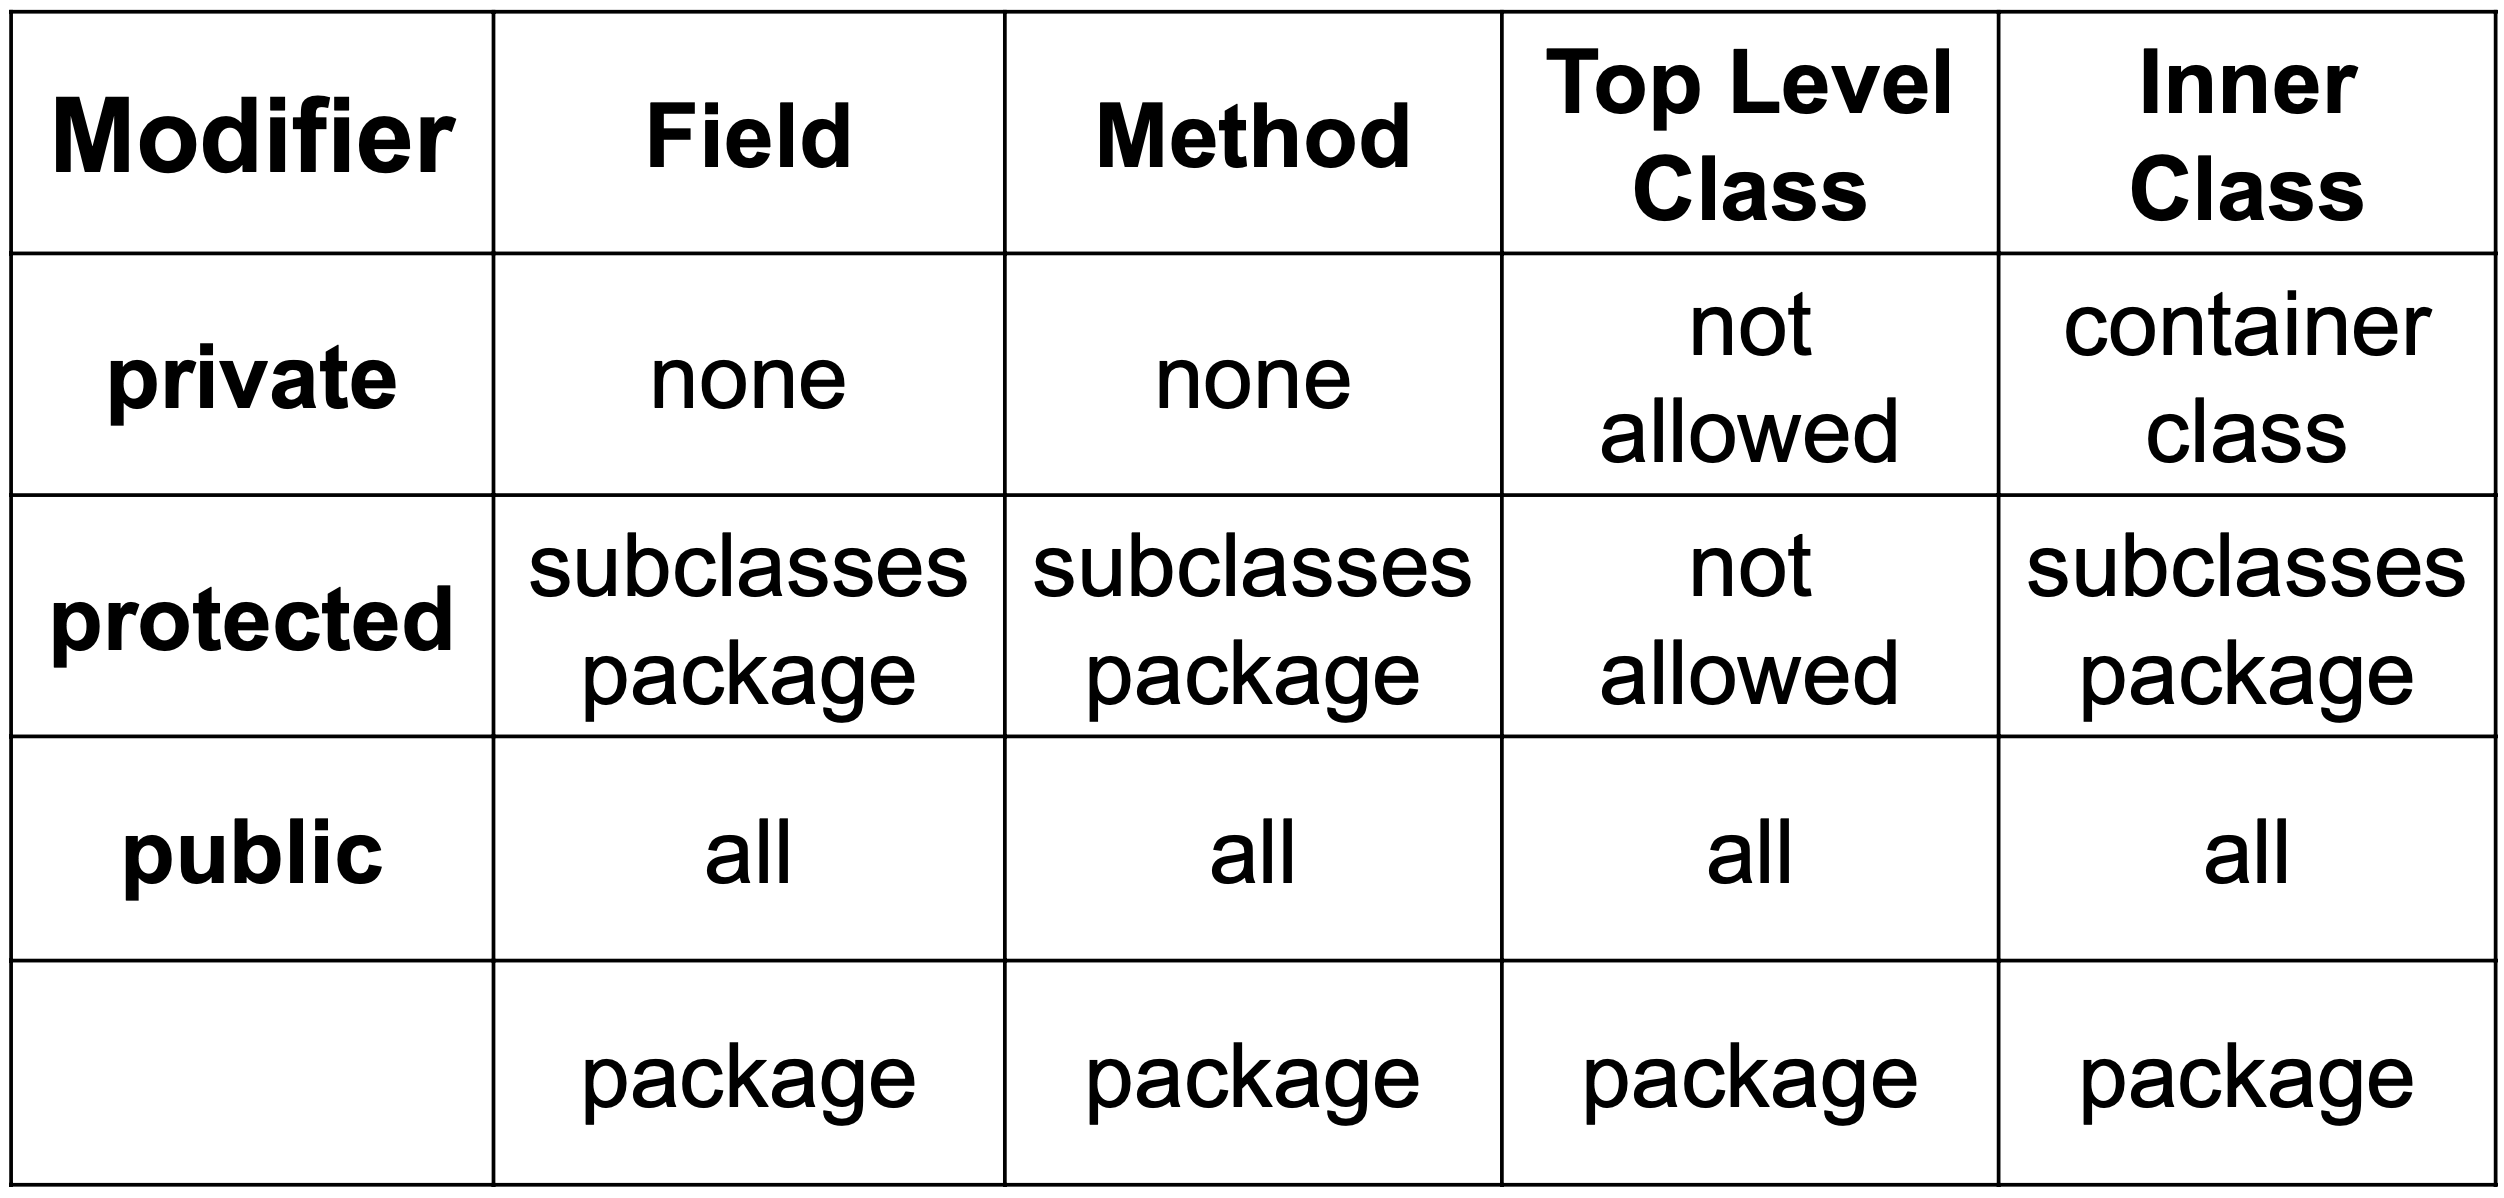
\includegraphics[width=0.6\linewidth]{res/java/VisibilityModifiers.png}
    \caption{Modificatori della visibilità}
\end{figure}
\subsubsection{Methods}
I metodi sono delle funzioni che eseguono determinate operazioni, permettendo il riutilizzo del codice. Accettano parametri e ne restituiscono altri.
I \textbf{costruttori} sono metodi speciali che creano istanze di classe. Una classe può avere più costruttori. Il nome è quello della classe. Se non sono definiti costruttori, viene utilizzato quello di default (vuoto), che viene invocato anche dalle subclasses.
Alcune convenzioni per i metodi:
\begin{itemize}
    \item Validare gli argomenti prima di utilizzarli: \textit{mai dare per scontato che l'utente non sia una scimmietta incazzata.}
    \item Utilizzare la keyword \code{final} per gli argomenti, in modo da non poterli modificare nel codice
    \item Spaziare gli argomenti nella lista. \textit{Ma non fate le bestie di satana mettendo lo spazio dopo la parentesi}
\end{itemize} 
\subsubsection{Fields and variables}
Le variabili forniscono spazio in memoria. Hanno un tipo specifico che determina la memoria occupata, i valori assumibili, le operazioni applicabili. Il loro scope dipende dal modifier associato. \textbf{Lo scope delle variabili locali inizia nel punto di dichiarazione e finisce con la fine del blocco dove sono state dichiarate.} A partire da Java10, in alcuni casi non è necessario dichiarare il tipo. \textit{/s Am I PHP-dreaming?}
\subsection{Static fields, methods, blocks}
Gli attributi/metodi statici esistono indipendentemente dagli oggetti. Possono quindi essere chiamati senza presenza di oggetti, ma con alcune restrizioni: possono chiamare solo metodi statici, possono accedere solo a campi statici, non possono usare this/super. Sono ovviamente condivisi tra tutte le istanze. Un blocco static viene caricato una sola volta quando una classe viene caricata. 
\subsection{Final classes, methods, fields}
Una classe dichiarata \code{final} non può essere estesa. Un metodo \code{final} non può essere overridato. Un field \code{final} non può essere modificato, è quindi costante. Va inizializzato alla dichiarazione, nei costruttori o in un blocco static. 
\subsection{Classe Serializable}
Una classe che implementa l'interfaccia \code{Serializable} deve rispettare uno di questi tre constraints:
\begin{itemize}
    \item Contenere dati primitivi
    \item Contenere oggetti Serializable
    \item Essere un transient 
\end{itemize}
\subsection{Oggetti immutabili}
I campi sono final, le subclasses non possono overridare metodi. I metodi non possono modificare gli oggetti mutabili collegati ai fields, in quanto non sono condivisi. 
\subsection{Coding Conventions}
Elenchiamo ora qualche coding convention.
\subsubsection{Field coding conventions}
\begin{itemize}
    \item Dichiarare i campi private per fornire incapsulamento
    \item Inizializzare i final all'interno dei costruttori
    \item Non inizializzare i campi numerici con \glspl{magic}, ma usare una costante
\end{itemize}
\subsubsection{Variable coding conventions}
\begin{itemize}
    \item Dichiarare le variabili appena prima del loro utilizzo
    \item Evitare l'assegnamento di più variabili allo stesso valore in un singolo statement
    \item Non utilizzare i \glspl{magic}
    \item Separare i membri in base al loro scope 
    \item Utilizzare nomi esplicativi
\end{itemize}
\subsubsection{JavaBean classes coding conventions}
\begin{itemize}
    \item Dovrebbero avere un costruttore vuoto
    \item Dovrebbero essere Serializable $\rightarrow$ supporta uno storing/restoring affidabile delle istanze 
    \item Dovrebbe avere getter/setter con una convenzione di nomi: getCampo, setCampo, o se boolean anche isCampo
\end{itemize}
\subsection{Ereditarietà}
L'ereditarietà è il meccanismo che permette di ereditare campi e metodi delle superclassi. Il vantaggio principale è il riutilizzo del codice. Le subclasses non possono usare i campi privati, ovviamente. Possono anche overridare i metodi non final. 
\subsection{Method overloading e overriding}
L'overloading avviene quando abbiamo più implementazioni dello stesso metodo, cambiando gli argomenti ma avendo ugual nome e return type. Un metodo è overridden quando una subclass ridefinisce un metodo con la stessa firma della classe padre. 
\subsection{Abstract classes}
Le classi astratte forniscono un'implementazione parziale. Dovrebbero avere solo costruttori \textit{protected}, possono includere metodi astratti. Se una classe ha metodi astratti, è astratta. Ma non è necessario.
\subsection{Interfaces}
Vi sono in realtà 3 definizioni di \textbf{interfaccia.}
\begin{itemize}
    \item Software systems: è un confine condiviso tra due componenti separati che scambiano informazioni. Lo scambio può essere tra software, hardware e umani. es. Interfaccia di rete.
    \item Software engineering: è un principio chiave di design che proibisce l'accesso alle risorse di default, permettendo l'accesso solo tramite entry point definiti. Sono delle specifiche verificabili (contracts) per componenti software, che estendono la definizione ordinaria di tipi di dati astratti tramite l'uso di constraints
    \item Object-oriented languages: è un tipo astratto che non contiene dati ma definisce comportamenti tramite le firme dei metodi (nome, argomenti, return type)
\end{itemize}
\subsubsection{Java interface}
In Java, le interface sono reference type simili alle classi, che inizialmente contenevano solo metodi astratti e costanti. Da Java8, può contenere metodi default e static con implementazione. I metodi default offrono un'implementazione utilizzata da più subtypes, che possono overridarli, a differenza degli static. Da Java9 le interfacce possono anche contenere metodi privati. Le classi possono implementare \textbf{una o più interfacce}, ereditandone i metodi astratti. Le interfacce possono anche estendere altre interfacce (anche multiple). Per questo, le classi sono meno estensibili: possono farlo con una sola classe.
\subsection{Ereditarietà e composizione}
Eredità e composizione definiscono relazioni tra due classi per ridurre la duplicazione di codice e i bug. L'ereditarietà forma una relazione di tipo \textit{is-a}, la composizione \textit{has-a}
\subsection{Marker interfaces e functional interfaces}\label{funcint}
Le \textbf{marker interfaces} sono interfacce vuote, ossia non contengono metodi e costanti. Le \textbf{functional interfaces} sono interfacce con un singolo metodo astratto.
\subsection{Inner classes}
Le \textbf{inner classes} sono classi definite all'interno di un'altra classe, e hanno 4 possibili tipi:
\begin{itemize}
    \item \textbf{Non-static inner class} possono accedere a tutte le istanze private della classe esterna
    \item \textbf{Local inner classes} sono classi non statiche definite all'interno di un metodo
    \item \textbf{Anonymous inner classes} sono classi non statiche definite senza nome, come subclass o implementazione di un'interfaccia
    \item \textbf{Static inner classes} non sono tecnicamente inner classes. Sono in realtà un membro statico dell'outer class. Sono meno agganciate alla classe esterna, il che aiuta la qualità del codice, il testing, il refactoring. È in realtà una classe top-level, implementata dentro un'altra per motivazioni di packaging.
\end{itemize}
\subsection{Enums}
Gli \textbf{enums} sono classi speciali rappresentanti gruppi di costanti. È l'abbreviazione di enumeration. È implicitamente final, quindi non può avere subclasses. Le costanti sono public static.
Gli enums possono essere definiti all'interno di una classe, possono contenere costruttori eseguiti separatamente per ogni costante. Può contenere solo metodi concreti (non astratti); può implementare più interfacce e dichiarare un main. 
\subsection{Annotations}
Le \textbf{annotazioni} forniscono informazioni supplementari riguardanti il software. Non ne modificano l'azione, ma aiutano ad associare informazioni ad elementi del programma. Non sono commenti puri, in quanto possono modificare il comportamento del compilatore o la reflection. 
Alcuni esempi:
\begin{itemize}
    \item \textbf{@Deprecated:} suggerisce che il metodo è deprecato ed è stato sostituito da una versione nuova
    \item \textbf{@FunctionInterface:} suggerisce che l'interfaccia è di tipo functional, e darà errore se non rispettato
    \item \textbf{@Override:} indica che il metodo è ereditato 
    \item \textbf{@SafeVarArgs:} sopprime i warning del compilatore quando i parametri sono generics. Non usabile con l'overridde
    \item \textbf{@SuppressWarnings:} sopprime warning generici
    \item \textbf{@Documented:} indica che l'annotazione va documentata
    \item \textbf{@Inherited:} indica che un'annotazione della superclass è ereditata da una subclass
    \item \textbf{@Repeatable:} indica che la stessa annotazione può essere applicata più di una volta sullo stesso elemento
    \item \textbf{@Retention:} indica la retention policy
    \item \textbf{@Target:} indica il tipo di item a cui un'annotazione può essere applicata
\end{itemize}
\subsection{Retention Policies}
La retention policy definisce quando le annotazioni verranno scartate. Abbiamo più tipi di retention policies:
\begin{itemize}
    \item RetentionPolicy.\textbf{SOURCE}: le annotazioni verranno tenute nella source, e scartate durante la compilazione. Permette, ad esempio, la creazione di file sorgente addizionali durante la compilazione
    \item RetentionPolicy.\textbf{CLASS}: le annotazioni verranno tenute durante la compilazione, ma scartate per il runtime. Permette, ad esempio, l'uso di librerie per la manipolazione del bytecode che accedono al bytecode e modificano classi esistenti o ne generano dinamicamente
    \item RetentionPolicy.\textbf{RUNTIME}: le annotazioni saranno disponibili anche alla JVM. Permette l'accesso alle annotazioni tramite Java reflection, può essere usata per dare istruzioni al programma associato
\end{itemize}
\section{J6 - Javadoc}
\textbf{Javadoc} genera documentazione di codice Java prendendo in input dei file sorgente. L'output generato è un set di file HTML, più pacchetti e file di anteprima. 
Alcune delle feature principali sono:
\begin{itemize}
    \item Combina il source code con la sua documentazione
    \item Facilita la sincronizzazione tra documentazione e codice
    \item Genera le specifiche API dal sorgente
\end{itemize}
L'approccio di Javadoc è molto semplice: sfrutta commenti con una sintassi specifica, aggiungendo la possibilità di integrare pagine HTML. 
Alcuni tag, per esempio, sono: \code{@author}, \code{@inheritDoc}, \code{@docRoot}. Abbiamo anche dei tag che fanno riferimento a risorse, ossia \code{@link}, \code{@linkplain} e \code{@see}.
\section{J7 - Generics}
I \textbf{generics} sono simili ai template di C++. Permettono a tipi predefiniti o user-defined di essere parametro di metodi, classi, interfacce. Dall'arrivo dei generics bisogna salvare tipi specifici nelle collection. Questo aggiunge stabilità al codice, rendendo i bug più visibili tramite type checks più stretti. Riduce anche la necessità di casting nel codice. Alcune convenzioni di naming:
\begin{itemize}
    \item K: key
    \item N: number 
    \item T: type
    \item V: value
    \item S, U, V: altri...
\end{itemize}
\subsection{Metodi generici}
I metodi generici sono metodi i quali parametri/return types possono essere generics. Hanno una sezione di type parameter delimitata da $<>$ che precede il return type. Ogni sezione contiene uno o più tipi, separati da virgole. Un metodo generico è dichiarato come ogni altro metodo. 
\subsection{Wildcards}
Una \textbf{wildcard} permette di usare più di un tipo di elementi all'interno di una collection. È un meccanismo atto a rendere possibile il cast di collections alla loro subclass/superclass. L'obiettivo è rendere possibile la lettura e l'addizione di una collection generica. 
Alcuni tipi di wildcard:
\begin{itemize}
    \item Unknown wildcards List$<$?$>$: identifica una lista di tipo sconosciuto. È possibile la sola lettura, gli elementi vengono trattati come oggetti.
    \item Extend wildcards List $<$? extends A$>$: identifica una lista di elementi che sono sottoclassi di A. È possibile leggere (trattando gli elementi come istanze di A) ma non aggiungere.
    \item Super wildcards List $<$? super A$>$: identifica elementi della classe A o superclassi di A. È sicuro inserire istanze di A o sottoclassi, ma si possono leggere gli elementi solo come oggetti.
\end{itemize}
\subsection{Generic Class Implementation}
Ogni classe generica ha una singola implementazione basata sul tipo di oggetto. L'operatore \code{instanceof} non può essere utilizzato con un tipo generico. I generic types non possono essere usati per creare costruttori generici. Non si possono creare array generici.
\section{J8 - Collection Framework}
Un framework è un environment di software, universale e riutilizzabile, che fornisce alcune funzionalità facenti parte di una piattaforma software più grande, che facilitano lo sviluppo di software. 
Il \textbf{collection framework} fornisce un'architettura per salvare e manipolare gruppi di oggetti. Include vari tipi di interfacce e classi, e supporta le tipiche operazioni necessarie: ricerca, ordinamento, inserimento, ecc...
\subsection{Iterator, Iterable, Collection}
L'interfaccia \textbf{Iterable} è l'interfaccia sorgente di tutte le collection, e ha un metodo che ritorna un \textit{Iterator}. L'interfaccia \textbf{Iterator} fornisce la possibilità di iterare gli elementi in avanti tramite l'uso di tre metodi per verificare la presenza di un elemento, spostarsi, e rimuovere. L'interfaccia \textbf{Collection} estende l'interfaccia \textit{Iterable}, ed è l'interfaccia implementata da tutte le classi del collection framework. Nonostante l'interfaccia fornisca i metodi che le collezioni avranno, alcuni non sono implementati da alcune classi(\textit{contraction}).
I suddetti tre metodi sono:
\begin{itemize}
    \item \textbf{hasNext()} ritorna vero se esiste un elemento dopo il corrente
    \item \textbf{next()} sposta l'iteratore al prossimo elemento. Se non esiste, throwa un'exception.
    \item \textbf{remove (E e)} rimuove l'elemento corrente. Può ovviamente essere chiamato una sola volta per elemento.
\end{itemize}
Le collection hanno alcuni metodi principali: 
\begin{itemize}
    \item \textbf{contains(Object o)} e \textbf{ContainsAll(Collection$<$?$>$ c)} restituiscono true se la collection contiene uno/tutti gli elementi
    \item \textbf{isEmpty()} restituisce true se la collection è vuota 
    \item \textbf{iterator()} restituisce un iterator 
    \item \textbf{size()} restituisce il numero di elementi contenuti
    \item \textbf{stream()} ritorna uno stream sequenziale della collection 
    \item \textbf{toArray()} ritorna un array di oggetti contenente gli elementi della collezione
    \item \textbf{toArray(T[] a)} ritorna un array del tipo richiesto, contenente gli elementi della collezione 
\end{itemize}
\subsection{Lists}
L'interfaccia \textbf{List} definisce una struttura dati che gestisce una collezione ordinata di oggetti che possono avere valori duplicati. La classe \textbf{ArrayList} usa un array dinamico per salvare gli elementi, mantenendo l'ordine di inserzione degli elementi. Non è sincronizzato e l'accesso agli elementi è randomico. La classe \textbf{LinkedList} usa una lista doppiamente linkata internamente, mantiene l'ordine di inserimento e non è sincronizzata. La manipolazione di elementi è veloce perché non è necessario shifting. La classe \textbf{Stack} fornisce una struttura Stack aka \gls{lifo}, estendendo la classe vector.
I principali metodi delle liste sono:
\begin{itemize}
    \item \textbf{add(E e), add(int index, E e)} e \textbf{addAll(Collection $<$? extends E$>$ c)} hanno un compito decisamente ovvio.
    \item \textbf{get(int index)} ha un compito altrettanto ovvio.
    \item \textbf{set(int index, E e)} setta l'elemento index al valore e. \textit{In effetti era abbastanza ovvio pure questo.}
    \item \textbf{remove(int index), remove(E e), removeAll(Collection $<$?$>$ c)} \textit{- chissà cosa faranno mai questi -} rimuovono uno o più elementi
    \item \textbf{indexOf(Object o)} e \textbf{lastIndexOf(Object o)} restituiscono l'indice a cui si trova un elemento, oppure -1 se non c'è.
    \item \textbf{subList(int fromIndex, int toIndex)} genera una sottolista tra \code{fromIndex} (compreso) a \code{toIndex}(escluso)
 \end{itemize}
 L'utilizzo degli ArrayList è ottimale quando l'accesso è randomico e si aggiunge/rimuove solo dalla fine. La LinkedList, invece, viene usata quando è necessario manipolare anche gli elementi all'interno della lista.
 \subsection{Sets}
 L'interfaccia \textbf{Set} rappresenta un set non ordinato di elementi, che non ci permette di inserire duplicati. La classe \textbf{HashSet} rappresenta una collezione che usa una hash table per il salvataggio; l'hashing è utilizzato per il salvataggio. Il \textbf{LinkedHashSet} mantiene inoltre l'ordine di inserimento. Il \textbf{SortedHashSet} rappresenta un set ordinato in ordine crescente. Il \textbf{TreeSet} utilizza un albero per salvare: è molto veloce. \textit{Se l'unico tipo di albero che ti viene in mente è quello sotto casa tua, fai una googlata: è roba figa e ti tornerà utile.} 
 Elenco ora i metodi principali dei set:
 \begin{itemize}
     \item \textbf{add(E e)} aggiunge un elemento se non è già presente, e ritorna true se ha fatto.
     \item \textbf{remove(Object o)} rimuove l'elemento e ritorna true se l'ha trovato
     \item \textbf{addAll(Collection $<$? extends E$>$ c)} costruisce l'unione tra i due set 
     \item \textbf{retainAll(Collection$<$?$>$ c)} costruisce l'intersezione dei due set
     \item \textbf{removeAll(Collection$<$?$>$ c)} costruisce la differenza tra i due set
 \end{itemize}
 Gli HashSet vengono utilizzati quando è necessario inserire, eliminare, localizzare elementi. Il TreeSet è molto utile quando è necessario attraversare gli elementi secondo un ordine. Il LinkedHashSet è una via di mezzo. In base alla dimensione, può essere più veloce aggiungere elementi ad un HashSet piuttosto che convertirlo in un TreeSet.
 \subsection{Maps}
L'interfaccia \textbf{Map} fornisce una struttura dati che contiene valori basati su chiave. Ogni coppia chiave-valore è detta \textbf{Entry}. Una Map contiene chiavi univoche. L'\textbf{HashMap} è una mappa non ordinata. La \textbf{LinkedHashMap} è l'implementazione di una mappa, eredita da HashMap ma mantiene l'ordine di inserimento. La \textbf{SortedMap} rappresenta un set di elementi in ordine crescente. La \textbf{TreeMap} è l'implementazione di Map e SortedMap, mantenendo ordine crescente. I metodi principali delle Map sono 
\begin{itemize}
    \item \textbf{put(K k, V v)} collega la chiave k al valore v. Se la chiave esiste, ne sovrascrive il valore.
    \item \textbf{get(K k)} ritorna il valore associato alla chiave, o null se non viene trovata
    \item \textbf{remove(Object k)} rimuove l'entry collegata. Se trovata, restituisce il valore, altrimenti null.
    \item \textbf{replace(K k, V v)} sostituisce il valore solo se la chiave viene trovata. Restituisce il valore precedente.
    \item \textbf{entrySet(), keySet(), values()} restituiscono rispettivamente le entry, le chiavi, i valori.
\end{itemize}
L'HashMap è ottimale quando è necessario l'inserimento, l'eliminazione, la localizzazione. La TreeMap è utile quando si necessita un'esplorazione ordinata delle chiavi. La LinkedHashMap è una via di mezzo. A volte, in base alla dimensione, può essere più veloce aggiungere elementi ad una HashMap piuttosto che convertirla ad una TreeMap ed aggiungerli poi.

\subsection{Queues}
L'interfaccia \textbf{Queue} mantiene l'ordine \gls{fifo}. Può essere definito come lista ordinata, ed è utilizzato per salvare elementi in attesa di processi. La \textbf{PriorityQueue} mantiene elementi che devono essere processari in base alla loro priorità; non ammette valori null. La \textbf{Deque} gli elementi possono essere aggiunti/rimossi da entrambi i lati. L'\textbf{ArrayDeque} e la \textbf{LinkedList} implementano la Deque interface. Questi sono i metodi principali:
\begin{itemize}
    \item \textbf{add(E e)} inserisce un elemento nella coda 
    \item \textbf{offer()} è preferibile ad add(E e), in quanto verifica di non violare restrizioni di capacità. Ritorna true in caso di successo.
    \item \textbf{peek()} prende il primo elemento della coda senza rimuoverlo. Se vuota, ritorna null.
    \item \textbf{element()} prende il primo elemento della coda senza rimuoverlo. Se vuota, throwa un'eccezione.
    \item \textbf{remove()} rimuove il primo elemento e lo restituisce. Se vuota, throwa un'eccezione.
    \item \textbf{poll()} rimuove il primo elemento e lo ritorna. Se è vuota, returna null.
\end{itemize}
La LinkedList è una normale coda FIFO. La PriorityQueue viene utilizzata quando è necessario un comparator.
\subsection{Collections Class}
La classe \textbf{Collections} fornisce un set di metodi statici per la creazione di implementazioni sincronizzate di collection, per la creazione di collection immutabili, per operazioni ricorrenti sulle collection.
Alcuni metodi:
\begin{itemize}
    \item \textbf{unmodifiableCollection(Collection$<$? extends T$>$ c)} ritorna una view non modificabile della collection. 
    \item \textbf{synchronizedCollection(Collection$<$T$>$ c)} ritorna una collection sincronizzata (thread-safe).
    \item \textbf{checkedCollection(Collection$<$E$>$ c, Class$<$E$>$ t)} ritorna una vista dinamica typesafe della collection. Ogni tentativo di inserimento di elementi incoerenti col type throwa exception.
    \item \textbf{singleton(T o), singletonList(T o), singletonMap(K k, V v)} restituiscono set, liste e mappe con elementi/key-values.
    \item \textbf{copy(List$<$? super T$>$ dest, List$<$? extends T$>$ src)} copiano tutti gli elementi di src in dest 
    \item \textbf{fill(List$<$? super T$>$ list, T obj)} riempe la lista con l'elemento specificato 
    \item \textbf{nCopies(int n, T o)} ritorna una lista immutabile con l'elemento fornito.
    \item \textbf{replaceAll(List$<$T$>$ list, T oldVal, T newVal)} restituisce tutte le occorrenze di un valore con l'altro 
    \item \textbf{reverse(List$<$?$>$ list)} inverte l'ordine degli elementi
    \item \textbf{reverse(List$<$?$>$ list, int distance)} inverte l'ordine fino alla distanza specificata
    \item \textbf{binarySearch(List$<$? extends Comparable$<$? super T$>$$>$ list, T key)} implementa una ricerca binaria. La lista deve ovviamente essere ordinata. Ritorna l'indice dell'oggetto. \textit{Se non sai cos'è una ricerca binaria googla anche questo. Tutta roba figa.}
    \item \textbf{frequency, min, max (Collection$<$?$>$ c, Object o)} restituiscono la frequenza dell'elemento, il minimo, e il massimo
    \item \textbf{indexOfSubList, lastIndexofSubList(List $<$?$>$ source, List$<$?$>$ target)} ritornano la posizione della sublist trovata, o -1 se non c'è. 
\end{itemize}
\section{J9 - Functional programming}
Ci poniamo ora una domanda: qual è la differenza tra programmazione imperativa e funzionale? 
La \textbf{programmazione imperativa} è un paradigma che utilizza degli \glspl{statement} per modificare lo stato di un programma. La programmazione funzionale, invece, tratta la computazione come valutazione di funzioni matematiche. Uno \textbf{\gls{statement}} assegna variabili, una \textbf{funzione} è eseguita per produrre un valore. Quindi, il focus della programmazione imperativa è \textit{come risolvere}, quello della funzionale è \textit{cosa risolvere}.
\subsection{Funzioni pure e di higher-order}
\textit{Come cazzo si traduce higher-order?} Le \textbf{funzioni pure} restituiscono lo stesso risultato quando ricevono gli stessi argomenti, e non causano effetti collaterali. Per questo, sono semplici da debuggare. Inoltre, non fanno \gls{mock}. Le \textbf{funzioni higher-order} \textit{(forse "di ordine maggiore"? Suona veramente male)} prendono funzioni come argomenti e/o ritornano funzioni come risultato. 
\subsection{Calcolo lambda}
Il suddetto venne sviluppato da Alonzo Church per studiare la computazione tramite funzioni. Dà, in sintesi, la definizione di cosa è computabile. È un \textit{framework teorico} per descrivere le funzioni, la loro valutazione è basata puramente su manipolazione sintattica di simboli e ricorsione. \textbf{Tutto} ciò che può essere computato tramite calcolo lambda è computabile, e offre la stessa \textit{definitional power} di una macchina di Turing. Il calcolo lambda è la base di tutti i moderni linguaggi di programmazione funzionale. 
Il functional programming presenta però alcune difficoltà:
\begin{itemize}
    \item Scrivere funzioni pure riduce la leggibilità del codice
    \item Scrivere programmi ricorsivi al posto di cicli potrebbe non essere semplice
    \item Scrivere funzioni pure è semplice, ma combinarle con altro software no
    \item I valori immutabili e la ricorsione potrebbero ridurre le performance
\end{itemize} 
\subsection{Espressioni lambda}
\textit{Questo è un bel mindfuck.} Le espressioni lambda sono metodi anonimi che possono implementare una functional interface. \textit{Non ricordi cosa siano? Rileggi \ref{funcint}}. Il loro tipo è il tipo dell'interfaccia che implementano, e possono essere usate ovunque ci aspettiamo functional interfaces. Possono accedere solo ai field della classe che le racchiude, e alle variabili locali del blocco che le racchiude, solo se \code{final}. Una lambda, in termini pratici, consiste di una lista di parametri, una freccia, un corpo.
\begin{center}
    \code{(parameters) $->$ \{statements\}}
\end{center}
Parametri e return types possono essere omessi se determinabili dal contesto.
Le lambda con una sola espressione possono omettere le graffe. Le lambda con un solo parametro possono omettere le tonde. Le lambda senza parametri devono però averle. 
Alcuni vantaggi delle espressioni lambda:
\begin{itemize}
    \item Supportano la programmazione funzionale 
    \item Permettono di scrivere codice più pulito e compatto 
    \item Permette di scrivere programmi paralleli
    \item Fornisce API più generiche, flessibili, riutilizzabili
    \item Supporta il passaggio di behavior a metodi
\end{itemize}
\subsection{Riferimenti ai metodi}
Spesso le lambda expressions chiamano metodi esistenti. Non è però conveniente e conviene chiamarlo direttamente. I riferimenti a metodi sono, effettivamente, una forma semplice di espressioni lambda. Possono essere utilizzati per metodi statici, di istanza, e costruttori. Ne abbiamo, di conseguenza, tre tipi:
\begin{itemize}
    \item Metodo statico: \code{ContainingClass::staticMethodName}
    \item Metodo di istanza: \code{containingObject::instanceMethodName}
    \item Costruttore: \code{ClassName::new}
\end{itemize}
\subsection{Streams}
Gli \textbf{streams} sono simili a collections, ma non mantengono i dati. Sono pensati per lavorare bene con le lambda expressions. Sono immutabili, ma processandoli ne possiamo ottenere nuovi. Muovono elementi lungo una sequenza di step di processo, detti \textit{stream pipeline}, formato da chiamate \textit{chaining} a metodi. La pipeline inizia con una sorgente di dati, esegue operazione intermedie, e conclude con un'operazione finale. Le operazione intermedie sono \textit{lazy}: non vengono eseguite fintanto che un'operazione da terminale lo richiede.
\subsubsection{Produrre streams}
Ci sono vari metodi per produrre stream:
\begin{itemize}
    \item Utilizzare il metodo statico \code{of} e passargli elementi/un array
    \item Convertire una collection utilizzandone il metodo \code{stream()}
    \item Convertire le linee di un file in stringhe, ed il file in uno stream di stringhe
    \item Ogni stream può essere convertito in uno stream parallelo usando il metodo \code{parallel()}
\end{itemize}
\subsubsection{Trasformare streams}
Abbiamo inoltre metodi di trasformazione degli streams:
\begin{itemize}
    \item Il metodo \code{map} trasforma uno stream applicandovi una funzione 
    \item Il metodo \code{filter} trasforma uno stream eliminando gli elementi che non soddisfano una condizione
    \item Il metodo \code{limit(n)} trattiene i primi n elementi
    \item Il metodo \code{skip(n)} rimuove i primi n elementi
    \item Il metodo \code{distinct} rimuove i duplicati 
    \item Il metodo \code{sorter} ordina gli elementi dello stream 
\end{itemize}
\subsubsection{Collectiong results}
Possiamo anche raccogliere determinati risultati:
\begin{itemize}
    \item \code{count}, \code{max}, \code{min}, \code{sum} restituiscono un singolo valore
    \item Il metodo \code{toArray} restituisce un array 
    \item Il metodo \code{collect} restituisce una lista o un set
    \item Il metodo \code{collect}, applicato ad uno stream di stringhe, riunisce tutte le stringhe in una sola
\end{itemize}
\section{J10 - Eccezioni}
\textbf{Eccezioni} ed \textbf{errori} sono eventi indesirati ed inaspettati che accadono durante l'esecuzione del programma, bloccando il normale flusso di esecuzione. Gli \textbf{errori} indicano problemi seri che non andrebbero \textit{catchati}. Le \textbf{eccezioni}, invece, possono essere "recuperate". Quando un'eccezione/errore accade, viene generato un oggetto e viene passato al \textit{runtime system} (aka la JVM). Questo oggetto contiene nome e descrizione dell'errore, e lo stato del programma quando è accaduto.
\subsection{Espressioni checked e unchecked}
Qual è la differenza? Le \textbf{eccezioni checked} rappresentano condizioni invalide in aree fuori dal controllo del programma: input dell'utente, database, rete, file mancanti. Queste sono sottoclassi di \code{Exception}, e i metodi sono obbligati a gestirle. Le \textbf{eccezioni unchecked}, invece, rappresentano difetti del programma, come argomenti invalidi passati ad un metodo. Queste sono subclasses di \code{RuntimeException}, ed i metodi non sono obbligati a gestirle. 
\begin{figure}[H]
    \centering
    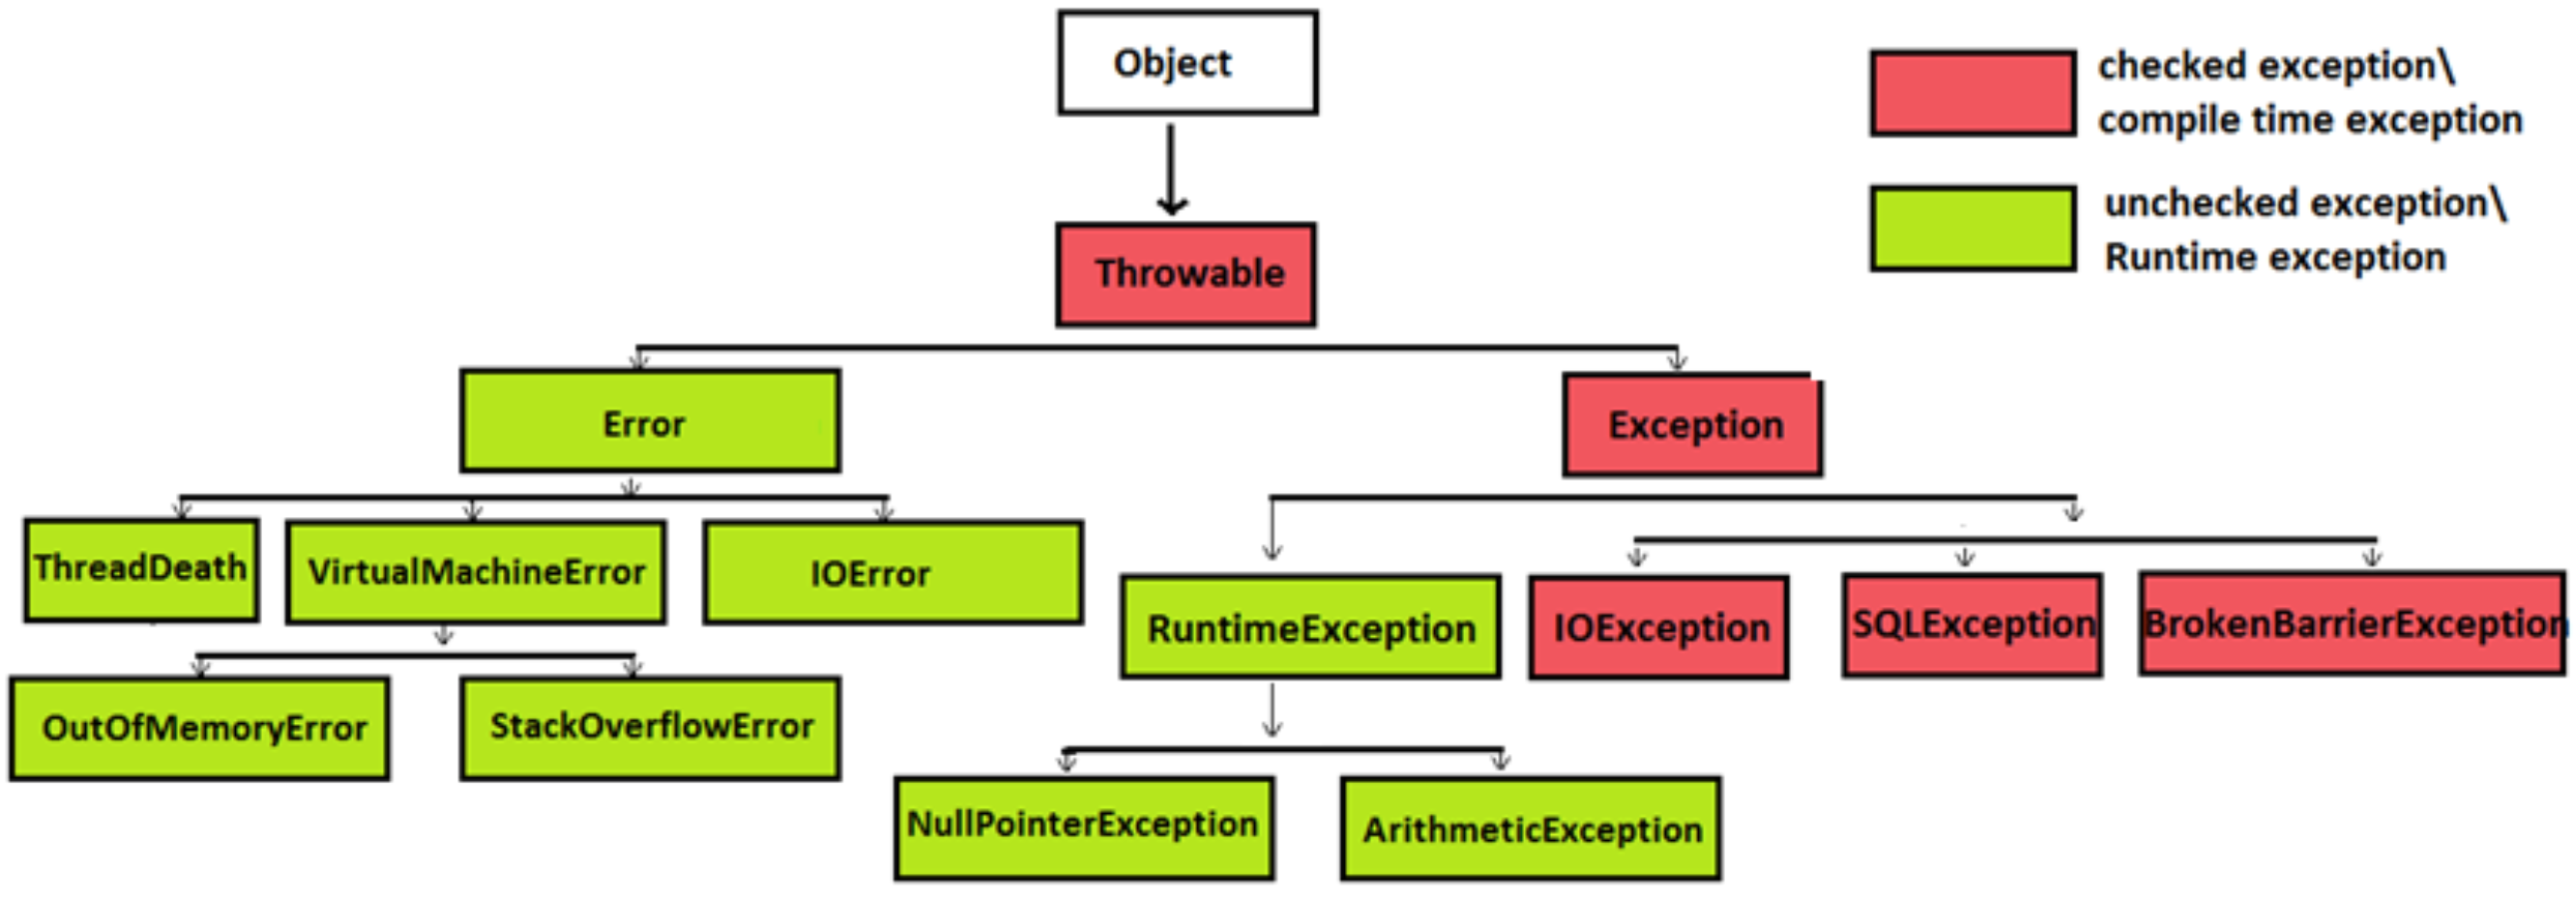
\includegraphics[width=0.8\linewidth]{res/java/Exceptions.png}
    \caption{Gerarchia delle eccezioni}
\end{figure}
\subsection{Exception handling}
Gli statement di un programma possono \textit{raisare} un'eccezione contenuta in un \textit{try block}. Se un'eccezione accade in un try block può essere \textit{caught} con un catch block. Bisognerebbe gestire tipi diversi di eccezioni in catch blocks diversi. Codice da eseguire in casi positivi e negativi va inserito in un finally block.
\subsection{Try with resources}
Generalmente, quando un try block utilizza risorse come file e connessioni, le suddette vanno chiuse in un finally block. Esiste però un metodo per non doverlo fare: dichiarare esplicitamente le risorse utilizzate tra parentesi prima del try block. La classe deve implementare l'interfaccia \code{AutoCloseable}.
\subsection{Throws e throw keyword}
Se il codice di un metodo può raisare \textit{(scusate)} eccezioni ma non vuole gestirle, può "throwarlo" al metodo padre inserendo \code{throws} nella sua firma. Invece, la keyword \code{throw}, solleva esplicitamente un'eccezione.
\subsection{Convenzioni di coding}
\begin{itemize}
    \item \textit{Questo lo abbiamo fatto tutti:} \textbf{evitare catch blocks vuoti.} Questo perché quando accade un'eccezione non ti rendi conto di nulla. Non è ok.
    \item Essere specifici nella \code{throws} dei metodi 
    \item Non raggruppare le eccezioni catchando una classe generica
\end{itemize}
\section{J11 - Input and Output}
\subsection{File class}
La classe \textbf{File} crea oggetti che forniscono una rappresentazione astratta di file/directory e ne supportnao la gestione. Supporta l'accesso agli attributi di file/directory, l'eliminazione, la rinomina, l'esplorazione di cartelle, i permessi.
\subsection{Streams}
Gli streams sono la classe principale del pacchetto \code{java.io}, e rappresentano sorgenti di input e destinazioni di output. Rappresentano diversi tipi di sorgenti/destinazioni, e supportano diversi tipi di dati. Possono passare dati ma anche manipolarli, e rappresentano la sequenza di dati letti/scritti da un programma. Due classi base: \code{InputStream} e \code{OutputStream}. In generale, si processano quattro tipi di dati:
\begin{itemize}
    \item Byte streams: 8-bit bytes; FileInputStream, FileOutputStream
    \item Character streams: 16-bit Unicode; FileReader, FileWriter
    \item Data streams: dati primitivi; DataInputStream, DataOutputStream
    \item Object streams: oggetti; ObjectInputStream, ObjectOutputStream
\end{itemize}
\subsection{Buffered streams}
I \textbf{buffered streams} leggono dati da un'area di memoria detta \textit{buffer}, l'API input nativa viene chiamata quando il buffer è vuoto. Per stream senza buffer, ogni richiesta I/O è gestita dal sistema operativo, perdendo in efficienza. I buffered stream compiono operazioni su stream di byte e caratteri, quindi solitamente wrappano byte/character streams.
\subsection{Espressioni regolari}
\textit{Prima o poi le dovrai imparare, eh.} Le \textbf{espressioni regolari} forniscono un metodo "scientifico" per identificare stringhe testuali utilizzando \textit{wild cards}. \textit{Skipperò le spiegazioni, ma se vi interessa consiglio \href{https://regex101.com}{Regex101}}.
\subsection{Scanner}
Lo \textbf{scanner}, definito in \code{java.util.Scanner}, è utilizzato per ottenere l'input di dati primitivi e stringhe. La sua funzionalità è basata su tre passi: lettura da fonte, identificazione dei dati tramite delimitatori, processazione. Spezza il suo input in \textit{token} utilizzando dei delimitatori, di default lo spazio.
\subsection{Standard streams}
Java fornisce il supporto per I/O standard dove il programma prende input da tastiera e produce output sullo schermo. Java fornisce tre stream standard:
\begin{itemize}
    \item \code{System.in} per l'input
    \item \code{System.out} per l'output
    \item \code{System.err} è utilizzato per l'output di errori prodotti dal software 
\end{itemize}
\subsection{Java NIO}
Un secondo metodo è il \textbf{New I/O}, che supporta un approccio buffer-oriented e basato sui canali per l'I/O, con supporto a file system e file handling. Venne sviluppato per fornire un supporto ad alta velocità, non-blocking fino a che i dati non sono caricati. Fornisce alcuni oggetti, detti \textbf{selectors}, utilizzati per monitorare i gli eventi dei canali attraverso un singolo thread. 
\subsubsection{NIO paths and files}
L'interfaccia \code{Path} rappresenta percorsi del file system, di tipo assoluto o relativo. Le istanze Path possono essere create utilizzando il metodo statico \code{get}, passando la stringa del path. La classe \code{File} fornisce metodi statici per manipolare file e directory.
\section{J12 - Concorrenza}
Il problema è sincronizzare le attività di un'applicazione che dovrebbero essere svolte parallelamente, evitando conflitti nell'uso di risorse. La soluzione? Multitasking, multithreading, multiprocessing. 
\subsection{Differenze tra processo e thread}
Un processo è un programma eseguibile, con il suo spazio di indirizzi, che esegue un programma, comunica con files, rete, e \textbf{può contenere più thread.} Un thread, invece, è uno stream di istruzioni eseguite in sequenza, che condivide lo spazio degli indirizzi con altri thread, eseguendo una parte di programma. Comunica con accesso condiviso ai dati. 
\subsection{Metodi principali di un thread}
\begin{itemize}
    \item \code{start()} avvia l'esecuzione del thread
    \item \code{run()} definisce la task del thread 
    \item \code{yield()} informa lo scheduler che il thread è a disposizione per concedere il suo uso corrente del processore
    \item \code{interrupt()} interrompe il thread 
    \item \code{setPriority()} imposta la priorità del thread 
    \item \code{sleep()} interrompe il thread per un determinato numero di millisecondi
    \item \code{wait()} interrompe il thread finché non viene risvegliato da un altro processo
    \item \code{notify()} e \code{notifyAll()} svegliano uno o tutti i thread 
    \item \code{wait()}, \code{notify()}, \code{notifyAll()} sono ereditati da Object 
\end{itemize}
\subsection{Variabili volatile}
La keyword \code{volatile} tenta di risolvere i problemi di visibilità di variabili. Tutte le modifiche su variabili volatili sono scritte immediatamente in memoria, tutte le letture sono svolte dalla memoria principale. Per questo, le variabili \code{volatile} sono più costose per la CPU. L'accesso a variabili volatili previene il riordinamento delle istruzioni, che viene normalmente svolto per migliorare le performance. 
\subsection{Problemi di atomicità}
Un esempio: \code{i++} sembra un'istruzione atomica, ma è in realtà composta da tre operazioni: lettura, modifica, scrittura. C'è quindi un problema quando diversi thread lavorano contemporaneamente sulle stesse risorse. 
\subsection{Synchronized methods}
Quando un thread sta eseguendo un metodo \code{synchronized} su un oggetto, tutti gli altri thread che invocano metodi sincronizzati sullo stesso oggetto vengono sospesi fino a quando non finisce. 
\subsection{Atomic object classes}
Le classi oggetto atomiche forniscono metodi \textbf{atomici}, quindi le loro istruzioni vengono eseguite insieme, o nessuna viene eseguita. Un metodo atomico modifica il suo oggetto senza effetti collaterali. Queste classi cono definite in \code{java.util.concurrent.atomic}, con i seguenti metodi principali:
\begin{itemize}
    \item \code{addAndGet()} aggiunge il valore passato al corrente
    \item \code{decrementAndGet()} decrementa il valore di 1
    \item \code{incrementAndGet()} incrementa il valore di 1
    \item \code{accumulateAndGet()} applica una funzione al valore corrente
    \item \code{lazySet(i)} setta il valore passato
\end{itemize}
\subsection{Classi principali della collection Concurrent}
\begin{itemize}
    \item \code{CopyOnWriteArrayList()} è un'implementazione backed-up della copy on write array
    \item \code{CopyOnWriteArraySet()} come sopra ma con set
    \item \code{ConcurrentHashMap()} è un'implementazione ad alta concorrenza, alta performance, backed up da un'hash table
    \item \code{LinkedBlockingQueue}, \code{ArrayBlockingQueue}, \code{PriorityBlockingQueue} attendono i dati 
    \item \code{DelayQueue} è una queue bloccante di elementi ritardati, dove un elemento può essere preso solo dopo la scadenza del ritardo
    \item \code{SynchronousQueue} è una coda bloccante in cui ogni inserimento attende una rimozione da un altro thread
\end{itemize}
\textit{Chiedo scusa per la poca chiarezza di quest'ultima subsection. Non ci si capisce un cazzo.}

\section{J13 - Sockets}
I \textbf{socket} forniscono un'interfaccia per programmare reti sul layer di trasporto, con un utilizzo simile all'I/O da file. L'utilizzo è indipendente dal linguaggio di programmazione. 
Distinguiamo tra TCP e UDP, con le loro caratteristiche: TCP è affidabile, ordinato, bidirezionale, UDP \textit{è una merda.} Il comportamento normale di un server con TCP è il seguente: viene eseguito su un computer specifico, ha un socket collegato ad una porta specifica, rimane in attesa di richieste di connessione, le accetta, e crea un nuovo socket per la connessione su un'altra porta. In Java, per server/client, è sufficiente creare un socket, creare gli streams I/O, comunicare, chiudere il socket. 
\subsection{Socket su UDP}
I socket su UDP non necessitano di un \textit{socket di benvenuto}, non hanno streams ma inviano pacchetti contenenti byte da estrarre. 
\subsection{Oggetti}
Per inviare oggetti è sufficiente utilizzare degli ObjectInputStream/ObjectOutputStream. 
\subsection{Eccezioni}
Vi sono vari tipi di eccezioni possibili:
\begin{itemize}
    \item \code{IOException} nell'apertura dello stream o del socket 
    \item \code{UnknownHostException} nell'apertura di un socket sul client 
    \item \code{SecurityException} quando è presente un security manager
    \item \code{ClassNotFoundException} leggendo un oggetto
\end{itemize}


\printglossary

\end{document}